\documentclass{beamer}
%
% Choose how your presentation looks.
%
% For more themes, color themes and font themes, see:
% http://deic.uab.es/~iblanes/beamer_gallery/index_by_theme.html
%
\mode<presentation>
{
  \usetheme{default}      % or try Darmstadt, Madrid, Warsaw, ...
  \usecolortheme{default} % or try albatross, beaver, crane, ...
  \usefonttheme{default}  % or try serif, structurebold, ...
  \setbeamertemplate{navigation symbols}{}
  \setbeamertemplate{caption}[numbered]
} 

\usepackage[english]{babel}
\usepackage[utf8x]{inputenc}

\title[Spectral Graph Theory Applications]{Group Research Meeting}
\author{Adwait Datar}
\institute{Technical University of Hamburg}
\date{$3^{rd}$ Feb,2020}

\begin{document}

\begin{frame}	
  \titlepage
\end{frame}

% Uncomment these lines for an automatically generated outline.
%\begin{frame}{Outline}
%  \tableofcontents
%\end{frame}

%%%%%%%%%%%%%%%%%%%%%%%%%%%%%%%%%%%%%%%%%%%%%%%%%%%%%%%%%%%%%%%%%%%%%
\begin{frame}{Problem}	
\begin{figure}
	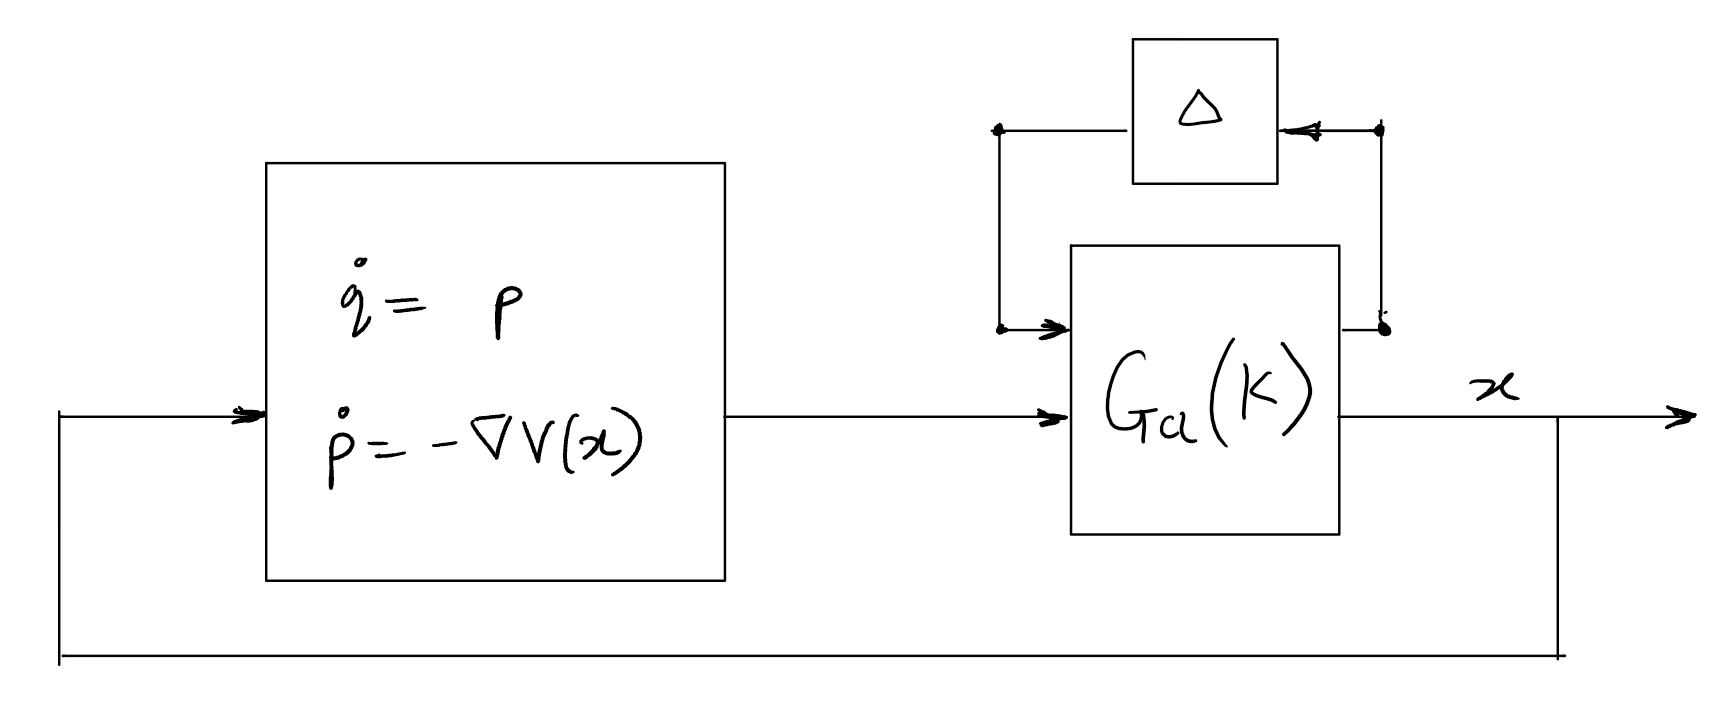
\includegraphics[width=1.0\linewidth]{figures/coupled_arch.JPG}
	\label{fig:mjlstraj}
\end{figure}
\begin{itemize}
	\item Coupled loop
	\item Two step-synthesis procedure:
	\begin{itemize}
		\item[1] Design a local tracking exponentially stabilizing controller (with performance measures specified by the exponents)
		\item[2] Use these as inputs to design the network dynamics
	\end{itemize}
	\item Analysis via
	\begin{itemize}
		\item rho-IQCs for exponential stability of tracking dynamics
		\item Singular perturbation theory
	\end{itemize}
	\item Numerically estimate(informally) the conservatism
\end{itemize}
\end{frame}
%%%%%%%%%%%%%%%%%%%%%%%%%%%%%%%%%%%%%%%%%%%%%%%%%%%%%%%%%%%%%%%%%%%%%%
%\begin{frame}{rho-IQCs\footnote{[2017] Boczar, Lessard, Packard, Recht}}
%\begin{minipage}{0.45\textwidth}
%	\begin{figure}
%		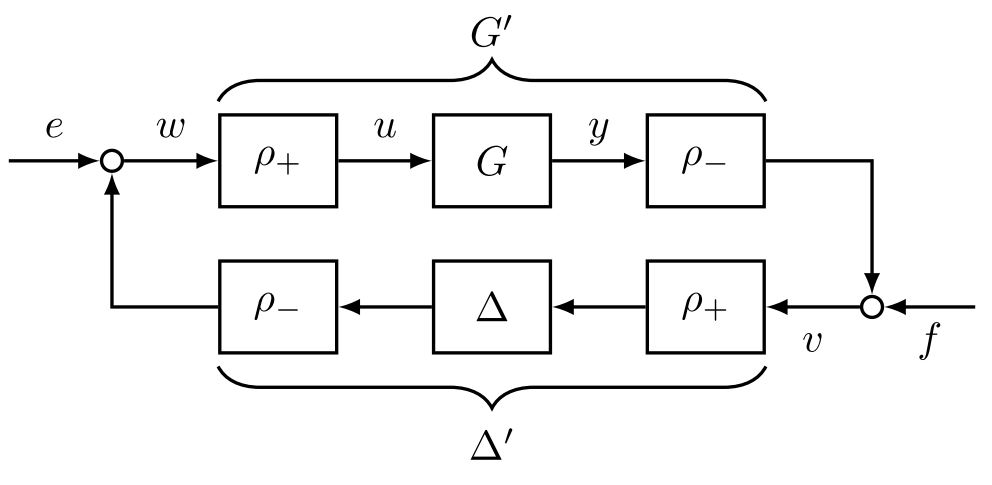
\includegraphics[width=1.0\linewidth]{figures/rho_IQCs.JPG}
%		\label{fig:mjlstraj}
%	\end{figure}
%\end{minipage}
%\begin{minipage}{0.45\textwidth}
%	\begin{figure}
%		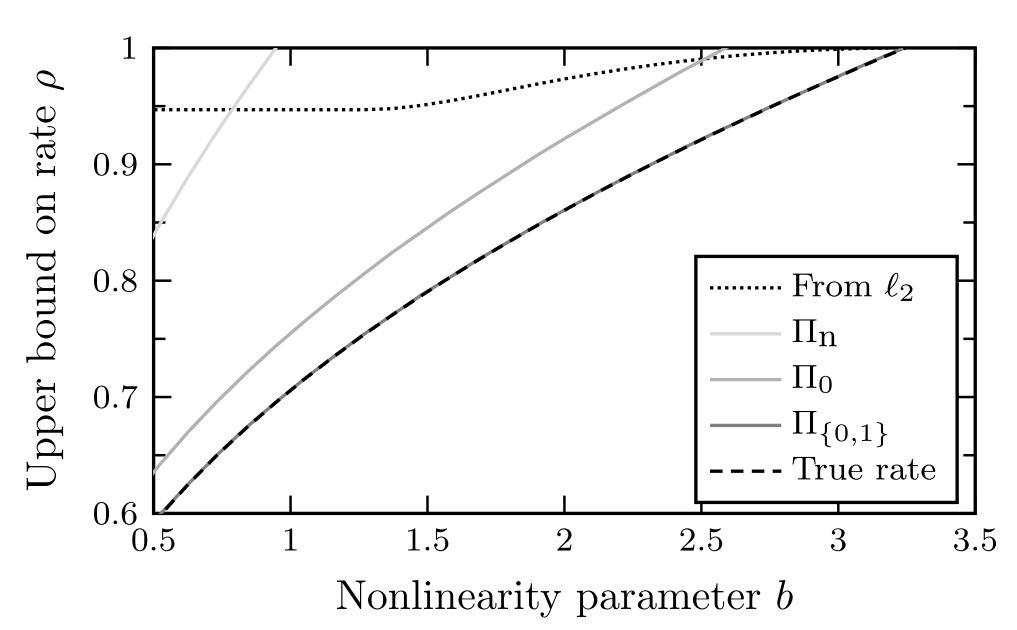
\includegraphics[width=1.0\linewidth]{figures/Conservatism_exponent.JPG}
%		\label{fig:mjlstraj}
%	\end{figure}
%\end{minipage}
%\begin{itemize}
%	\item L2/l2 gains give conservative bounds on the exponents 
%	\item Less conservative LMI formulations via rho-IQCs
%\end{itemize}
%\end{frame}
%%%%%%%%%%%%%%%%%%%%%%%%%%%%%%%%%%%%%%%%%%%%%%%%%%%%%%%%%%%%%%%%%%%%%


\begin{frame}{Time-scale separation\footnote{[2019] Awad ,Chapman , Schoof , Narang-Siddarth, and Mesbahi}}
	\begin{minipage}{0.45\textwidth}
		\begin{figure}
			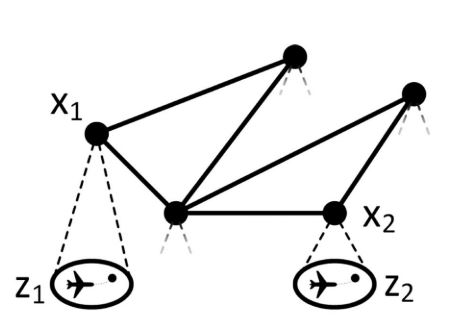
\includegraphics[width=0.6\linewidth]{figures/Time_scale_separation.JPG}
			\label{fig:mjlstraj}
		\end{figure}
	\end{minipage}
	\begin{minipage}{0.45\textwidth}
		\begin{figure}
			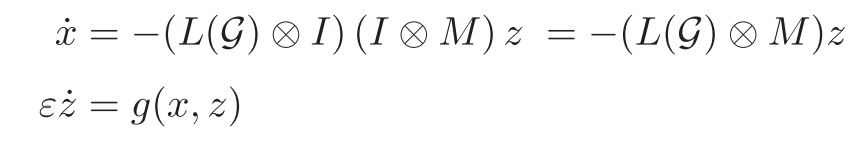
\includegraphics[width=1.35\linewidth]{figures/Time_scale_sep_dyn_sys.JPG}
			\label{fig:mjlstraj}
		\end{figure}
	\end{minipage}	
	\begin{itemize}
		\item If the time-scales are separated enough, we can study(and use the vast literature on) 
		\begin{itemize}
			\item simplified network dynamics
			\item robust/LPV controller synthesis for uncertain/non-linear agent dynamics
		\end{itemize}
	\end{itemize}
\end{frame}
\begin{frame}{Updates}
	\begin{itemize}
		\item Vidyasagar: Review singular perturbation for Linear systems
		\item Khalil: 
		\begin{itemize}
			\item Understand stability analysis
			\item Exponential stability relaxes the conditions on Lyapunov functions 
		\end{itemize}
		\item Ongoing work:
		\begin{itemize}
			\item Arrive at LMIs to search for Lyapunov functions
			\item Check the conservatism for simple examples
		\end{itemize} 
	\end{itemize}
\end{frame}
%%%%%%%%%%%%%%%%%%%%%%%%%%%%%%%%%%%%%%%%%%%%%%%%%%%%%%%%%%%%%%%%%%%%%%
%\begin{frame}{Starting Example}
%	\begin{figure}
%		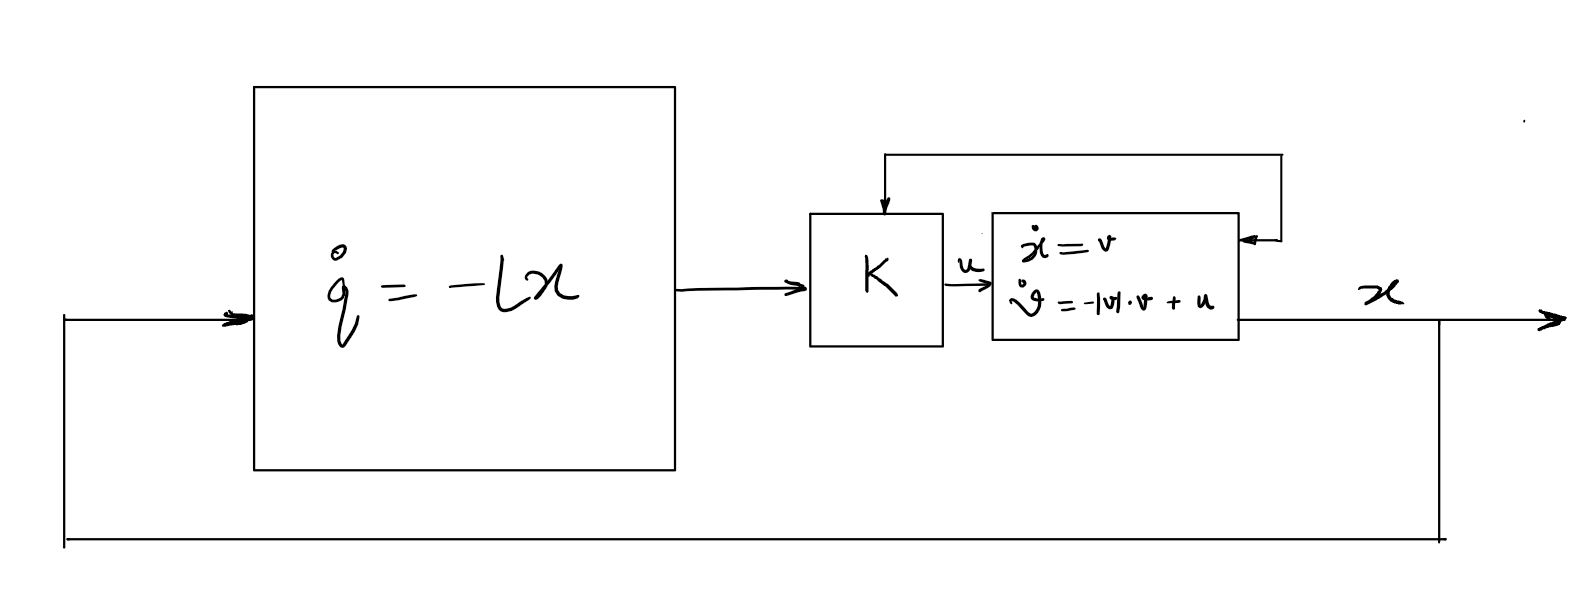
\includegraphics[width=1.0\linewidth]{figures/Starting_example.JPG}
%		\label{fig:mjlstraj}
%	\end{figure}
%	\begin{itemize}
%		\item First order consensus at the network level
%		\item Possible options local agent dynamics:
%			\begin{itemize}
%				\item LTI model with uncertain parameter
%				\item Damping coeff $b=|x|$ non-linearity (=sector non-linearity?)
%				\item Force saturation non-linearity (=sector non-linearity?)
%			\end{itemize} 						
%	\end{itemize}
%\end{frame}
%%%%%%%%%%%%%%%%%%%%%%%%%%%%%%%%%%%%%%%%%%%%%%%%%%%%%%%%%%%%%%%%%%%%%
\begin{frame}{Problem 2: Stochastic version of the IQC result}
\begin{minipage}{0.45\textwidth}
\vspace{4cm}
\end{minipage}
\begin{minipage}{0.45\textwidth}
	\begin{figure}
		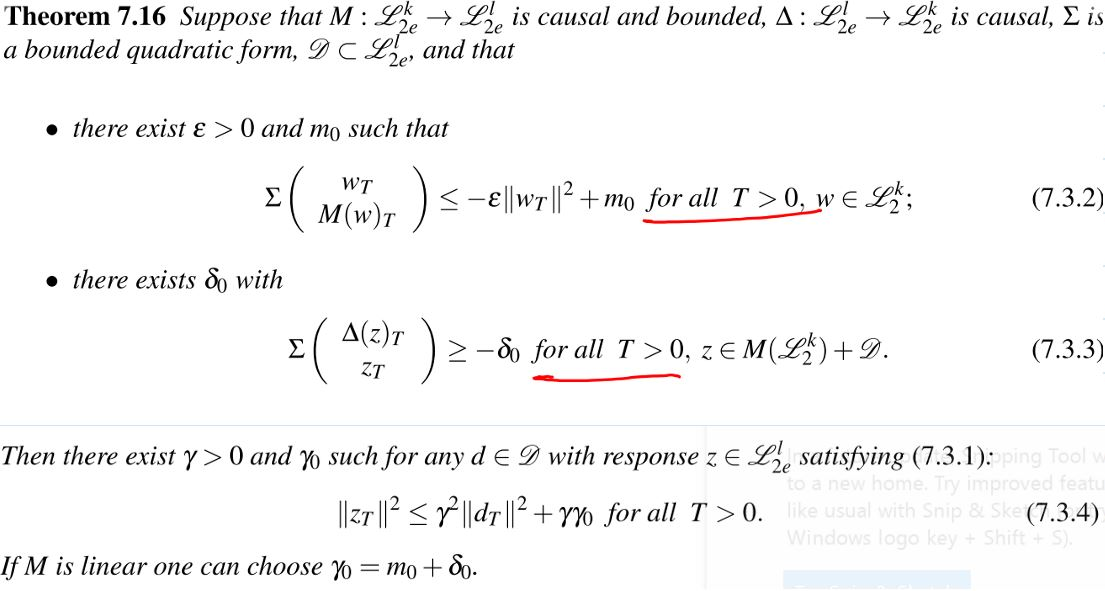
\includegraphics[width=1.35\linewidth]{figures/hard_IQC_theorem.JPG}
		\label{fig:mjlstraj}
	\end{figure}
\end{minipage}	
\begin{itemize}
	\item $\Delta$ is characterized by (7.3.3). Can we relax this to a stochastic version? 
\end{itemize}
\textbf{Updates:}
\begin{itemize}
	\item Understand the proofs and subtleties involved in hard and soft IQCs
\end{itemize}

	
\end{frame}
%%%%%%%%%%%%%%%%%%%%%%%%%%%%%%%%%%%%%%%%%%%%%%%%%%%%%%%%%%%%%%%%%%%%%
\begin{frame}{}
\begin{center}
    \huge{Thank you}
\end{center}
\end{frame}
%%%%%%%%%%%%%%%%%%%%%%%%%%%%%%%%%%%%%%%%%%%%%%%%%%%%%%%%%%%%%%%%%%%%%

\end{document}
